% Template for ICASSP-2015 paper; to be used with:
%          spconf.sty  - ICASSP/ICIP LaTeX style file, and
%          IEEEbib.bst - IEEE bibliography style file.
% --------------------------------------------------------------------------
\documentclass{article}
\usepackage{spconf,amsmath,graphics}

% Title.
% ------
\title{WAVELET SCATTERING REPRESENTATIONS \\*
FOR CLASSIFICATION OF HISTOLOGY IMAGES}
%
% Single address.
% ---------------
\name{Prashant Serai, Mark Rubeo, Peter Plantinga}
\address{The Ohio State University}
%
\begin{document}
%\ninept
%
\maketitle
%
\begin{abstract}
We use the Wavelet Scattering Convolution Network (ScatNet), as defined in Bruna
and Mallat (2013), to build invariant representations of microscopic images of breast
tissue. We then classify the image segments as containing primarily epithelium or stroma.
We evaluate multiple systems, and achieve results comparable to a strong baseline. Some
of our systems surpass the accuracy of a best-effort classification of the data by our
group members.
\end{abstract}
%
\begin{keywords}
image invariants, scattering transform, convolution network, medical image analysis
\end{keywords}
%
\section{INTRODUCTION}
\label{sec:intro}

Breast cancer is one of the leading diseases in the world, and it leads to nearly a
million deaths a year across the world. The most common diagnosis method for breast
cancer involves microscopic examination of the breast tissues. Currently, this is a
labor-intensive manual process. Motivated both by cost-saving and by potential
elimination of human error, research efforts are ongoing to automate as well as improve
the diagnosis process. An important sub-problem in automatic diagnosis pipelines is
classifying portions of images as mostly \emph{epithelium}, lining and surface cells,
or \emph{stroma}, connective cells \cite{Beck2011}.

\section{DATASET}
\label{sec:data}

Microscope slide images are often large and contain many regions of both epithelium
and stroma, and also regions that are distorted and not of interest. As part of the
diagnosis pipeline, the digitized slide is segmented into small images, also called
\emph{super-pixels}. We address the task of classifying whether these super-pixels
predominantly contain stroma or epithelium. Segmented images were graciously provided
by Raghu Machiraju’s research group at the Ohio State University. The images had been
hand-labeled by researchers trained in the task. Clear examples of epithelium and
stroma can be found in \textbf{Figure 1}, as well as an example that has a well-balanced
proportion of both epithelium and stroma, and is therefore difficult to classify,
even for humans.

We evaluated two datasets, one set containing smaller largely unambiguous 80 x 80
pixel images and the other set containing larger images of varying sizes. We had 600
of the 80 x 80 images, and 734 of the larger ones, with an equal distribution of
images labelled epithelium or stroma in both. Near perfect classification on the
smaller images was easily obtained and lot of the work focused on the dataset with
the 734 variably sized superpixels. We held out 100 randomly-selected images from
the super-pixels as the test set, and used the remaining 634 for training and
cross-validation tuning of hyper-parameters.

\section{SCATNET}
\label{sec:scatnet}

Each image contains a large amount of data, across all the pixels. Often, we care
only about certain "important" aspects of the information in the image, which can
be represented compactly. These features should be invariant to transformations such
as translation, rotation, scale, and so on. For example, in this application, the
position at which epithelial cells are located in the image is irrelevant, and their
orientation is also irrelevant.

Transformations such as SIFT \cite{Lowe1999} provide some invariant properties and a
compact representation of key information. However, in a hypothetical scenario, we may
also want to control the degree to which we want our output to be invariant to such
transformations. The transform described by Beck et. al. \cite{Beck2011}, generates a
compact representation of the image, and provides control for the degree of invariance
desired. Bruna and Mallat \cite{Bruna2013} suggest that for complex structures over
large domains, locally invariant information from SIFT, etc. is insufficient. They
say that the Scattering Transform provides not only SIFT-like descriptors at the
output of Layer 1, but also higher order information at the further layers, which
can help discriminate such complex structures. 

\begin{figure}
	\centering
	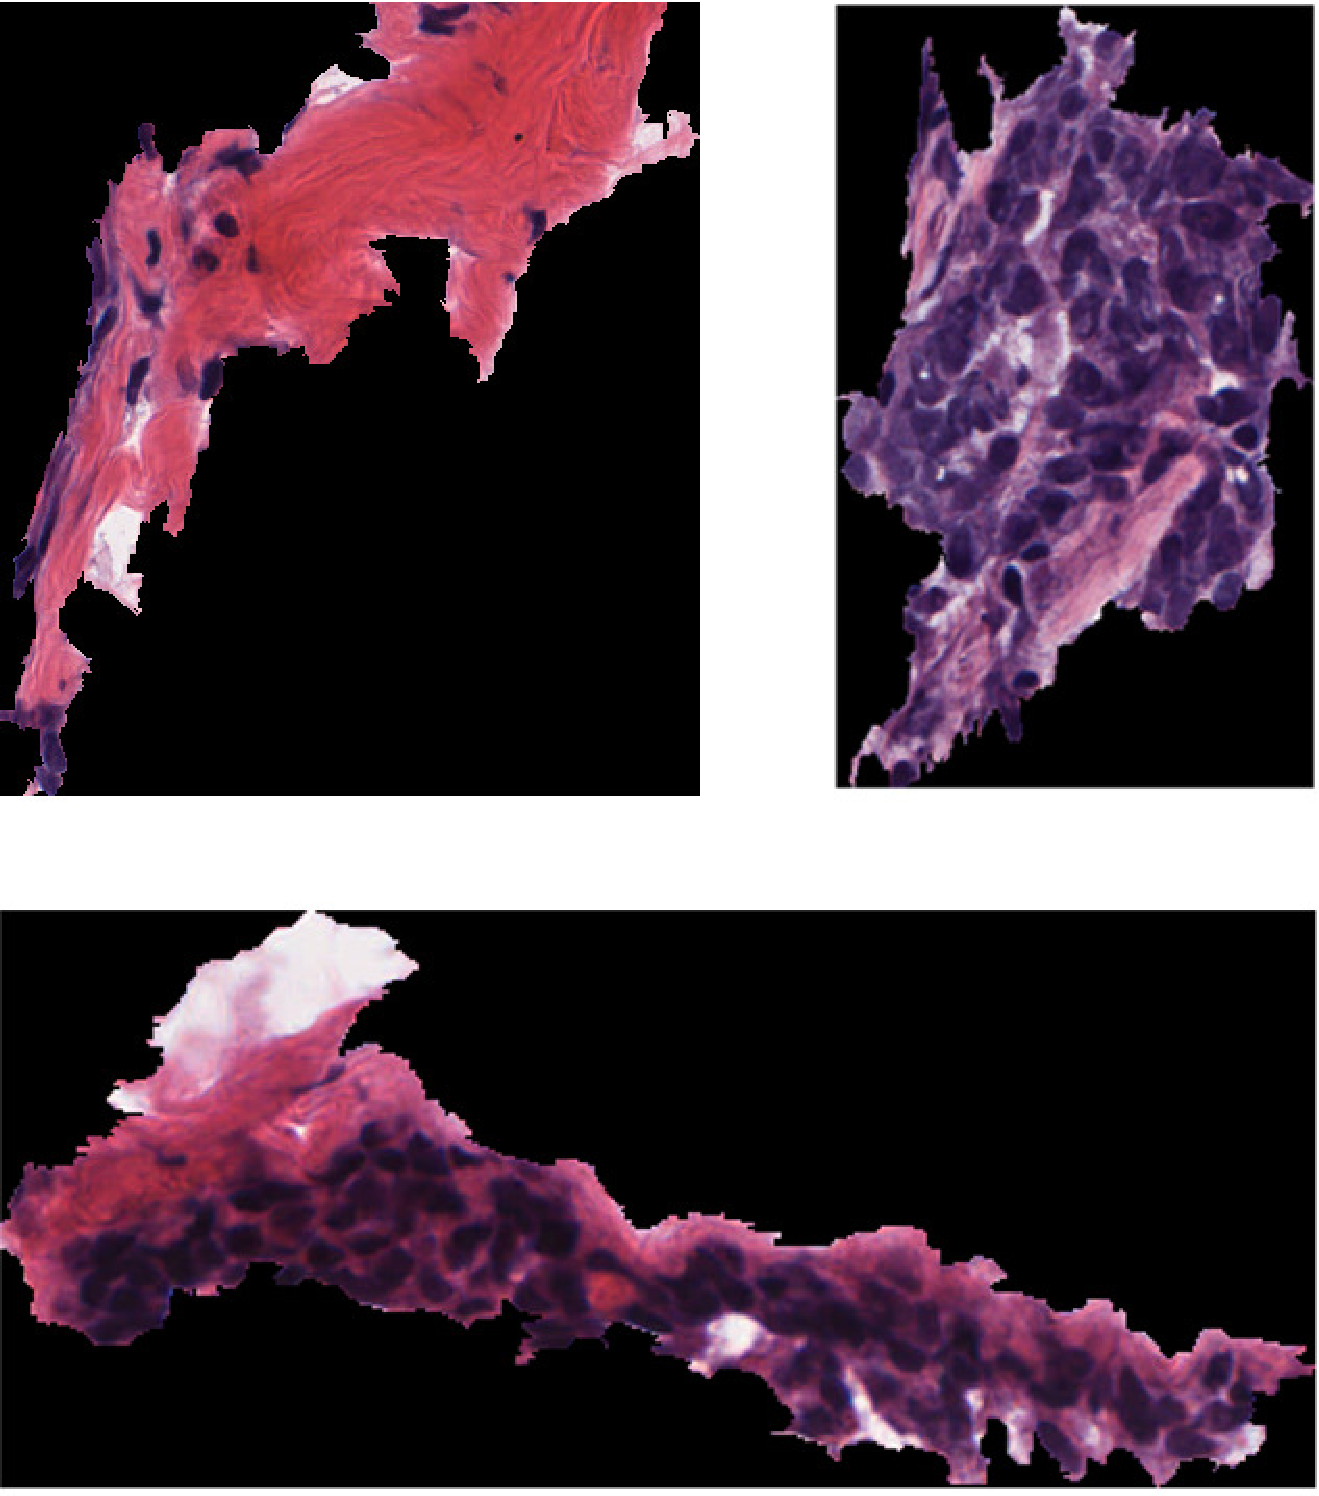
\includegraphics[width=0.45\textwidth]{images-mashup}
	\caption{Clockwise from top left -- super-pixels containing stroma, epithelium,
		and a mixture of both	(labeled stroma)}
\end{figure}

\begin{figure*}[b]
	\centering
	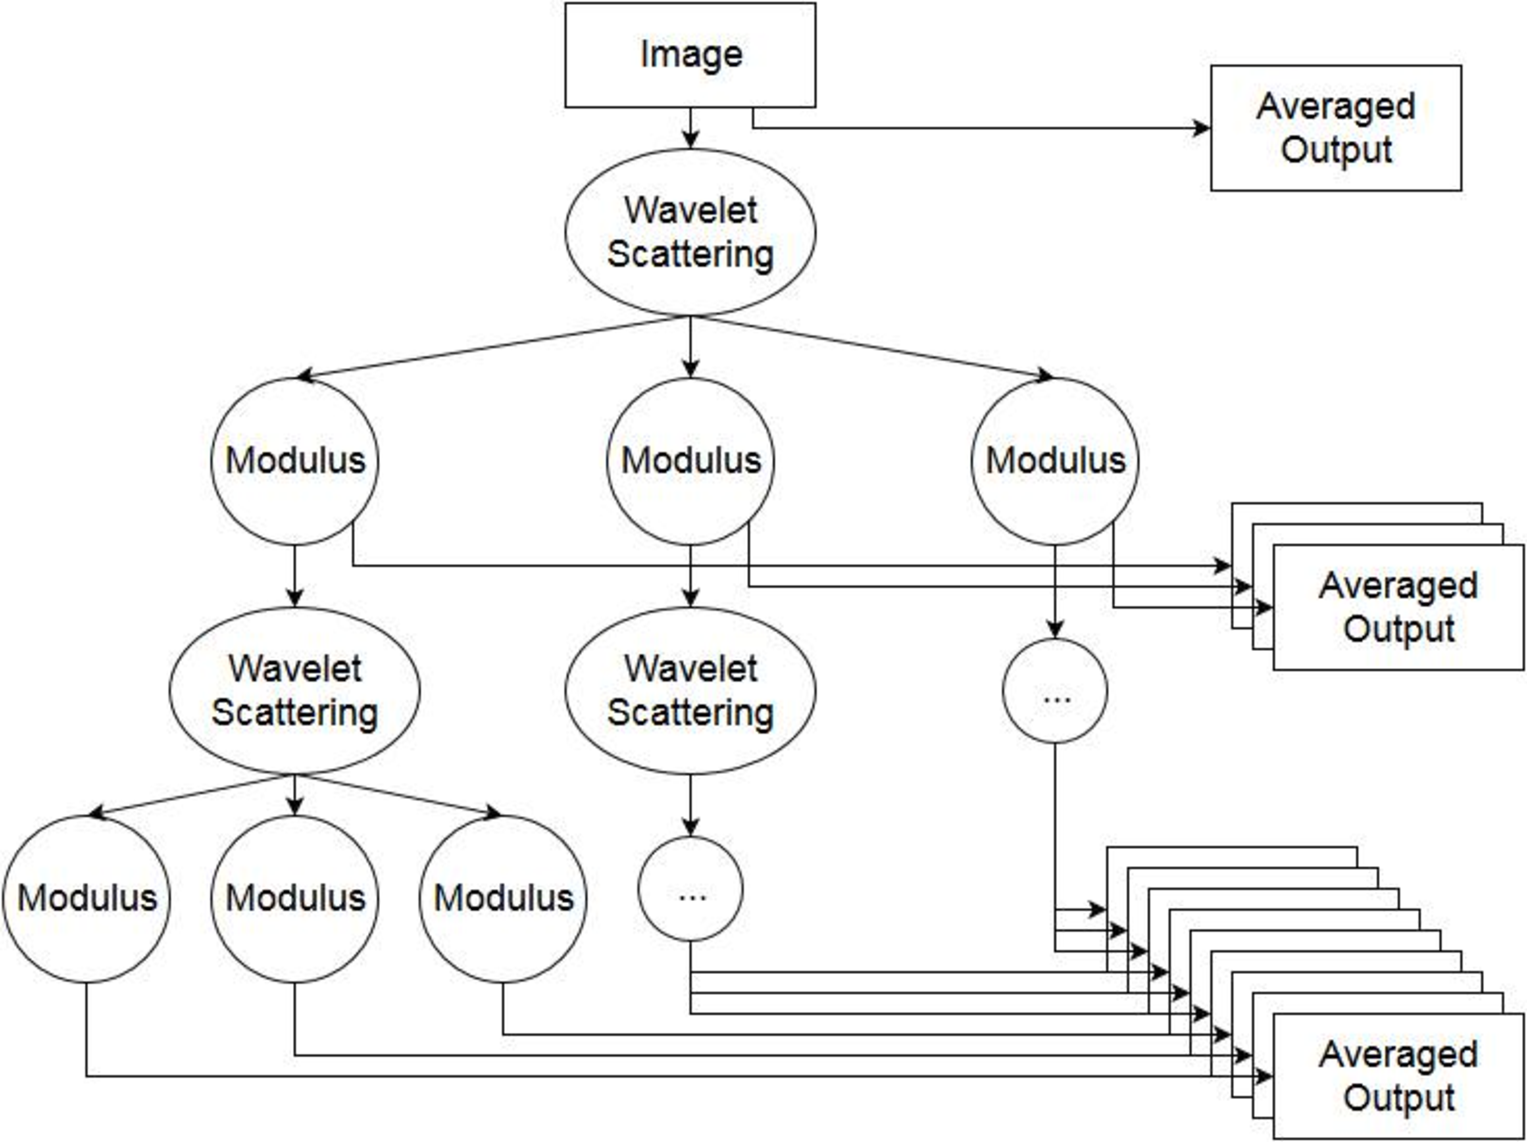
\includegraphics[width=0.8\textwidth,height=4in]{scatnet-process}
	\caption{ScatNet process. The output is the concatenation of all averaged moduli.}
\end{figure*}

The scattering transform is similar to the form of a deep convolution network with
wavelets being the convolving functions at each node. As in \textbf{Figure 2}, at each
layer, the input from the previous layer is convolved with wavelets at different scales and
orientations. This is essentially doing a complex wavelet transform, where the
information from the Image signal is divided in the complex frequency plane.
\cite{Kingsbury2001} The  number of divisions along the radial axis, $J$, and $L$,
the number of divisions along the rotational axis, are both configurable. Since
the outputs are taken through averaging filters, in order to get the desired invariant
properties, some high frequency information is lost. To recover the same, the
un-averaged information is passed to the next layer, where it is again convolved
with the wavelet filters. All the outputs are finally combined to form a feature
vector. Since, the feature vector contains correlated values, a classifier based
on affine principal component analysis (PCA) is used. It computes a transformation
to de-correlate the values and reduce the dimensionality to $N$, for each class, in
this case epithelium and stroma. The classification is done by looking at which
class' transformation minimizes the approximation error. More details about the
scattering transform, as well as the affine PCA classification technique are available
in Bruna and Mallat \cite{Bruna2013}. 

ScatNet also allows configurability of the number of layers, $M$, the number of scales
per octave in the wavelet transform; Q, the amount of oversampling carried out before
each layer; and the dimensionality of the affine PCA classifier $N$. After exploratory
preliminary testing, we tried all configurations of $J$ = 4, $L$ = 3 to 6, $Q$ = 1 to
10, $M$ = 1 to 4, $oversampling$ = 1 to 2, and $N$ = 2 to 20. Of the two best performing
configurations, we randomly re-partitioned the training 10 times and took the average,
finding the highest-performing configuration to be $J$ = 4, $L$ = 6, $Q$ = 1, $M$ = 3,
$oversampling$ = 1, $N$ = 2. 

ScatNet works with grayscale images and expects the images to be uniformly sized
and rectangular. Our data, however, is colored and has wide variation in image sizes
and aspect ratios, and the segments aren't rectangular. Further, the staining process
causes color to contain valuable information:  stromata stain a dull pink, while
epithelial cells stain a deeper purple. Our solution involves transforming the image
from RGB space to HSV (Hue-Saturation-Value) space, and compute the feature vector
independently for each color plane, eventually concatenating the 3 vectors to make 
the final feature vector. To account for the varying image sizes and non-rectangular
segments, we normalize the final feature vector, dividing it by the number of non-zero
pixels in the input image.

\begin{table}
	\begin{tabular}{c | c}
		\multicolumn{1}{c}{Hyperparameters} & Performance \\ \hline
		$J$ = 4, $L$ = 5, $Q$ = 1, $M$ = 3, $o.s.$ = 1, $N$ = 15 & 84.2\% \\
		$J$ = 4, $L$ = 6, $Q$ = 1, $M$ = 3, $o.s.$ = 1, $N$ = 2 & 87.2\% \\
	\end{tabular}
	\caption{Results for hyper-parameter configuration that achieve optimal results
	in exhaustive search}
\end{table}


\section{BASELINE SYSTEM}
\label{sec:baseline}

As a baseline, we applied a standard computer vision technique referred to as
 \emph{bag-of-visual-words} \cite{Csurka2004} \cite{Yang2007}. This technique 
involves finding points of interest (called  \emph{keypoints}) and some useful
information about them (called  \emph{descriptors}) and classifying based on the
similarity of these descriptors. We evaluated two well-known algorithms to
detect and describe keypoints: Speeded-Up Robust Features (SURF) \cite{Bay2008}
and Scale-Invariant Feature Transform (SIFT) \cite{Lowe1999}.

Both SIFT and SURF keypoint detection algorithms generate a few hundred keypoints
for each image. These usually occur in areas of high contrast, such as edges and
corners. Then, for each keypoint, these algorithms calculate a descriptor that
is designed to be invariant to scale, rotations, deformations, and other distortions.
For each keypoint, SURF gives a vector of 64 values, whereas SIFT gives a vector
of 128 values.

If we directly used the SIFT and SURF descriptors as features, the feature vector
length would be variable, since these algorithms generate a variable number of
keypoints. To deal with this, we clustered the keypoints to create a vocabulary
of “visual words”. For this step we used the most significant 20\% of all the
keypoints (based on the magnitudes of the descriptors) to find distinctive 
visual words. The number of clusters 'k' was empirically chosen to be 500,
with each cluster corresponding to one visual word in our vocabulary. These two
parameters are stable over a large range of values: varying the number of means
(from 30 to 10,000) and the percentage of descriptors kept (from 1\% to 80\%) showed no
significant differences in accuracy.

Finally, we calculated a bag-of-words feature vector for each image in both the
training set and the test set by counting the number of occurrences of each
visual word. This was done by finding all keypoints in each image and mapping
the descriptors to the closest mean. Each descriptor counts as an occurrence of
the associated word. Note that all descriptors are used at this stage, unlike at
the clustering stage. The bag-of-words features are then used to train an SVM
classifier to predict the class of the image.

Since the vanilla SIFT and SURF operate only on grayscale images, we tried two
methods to improve accuracy by using color information. First, we tried
decomposing the color image into three layers based on the HSV model of color,
and we generated keypoints for all three layers, clustering and classifying as
before. Second, we tried appending average hue and saturation to the feature
vector for the grayscale version of each image. There was no significant difference
in accuracy between these two methods.

\section{ALTERNATIVE BASELINES}
\label{sec:alternative}

We also present human evaluation and a simple 2-feature system as alternative
baselines. For the first, without formal instruction, we trained ourselves to
identify epithelium and stroma by inspecting images in the training set. We 
then evaluated our ability to classify 50 randomly-selected images of the 100 in
the test set.

While we are not experts at identifying stromata or epithelial cells, there are
two reasons that this baseline is informative. First, we are training ourselves
using exactly the same information that the computer has available to it: the
images in the training set. Second, we suspect that the images are at best very
hard to identify and at worst mislabeled. This baseline gives an impression of
how good we should expect the best systems to perform. 

Our second alternative baseline calculates two features for each image: average
hue and average saturation. Then we train a gaussian mixture model (GMM) using
expectation maximization. The resulting system performs surprisingly well,
indicating that a great deal of information is contained within the color
from the staining process.

\begin{figure}
	\centering
	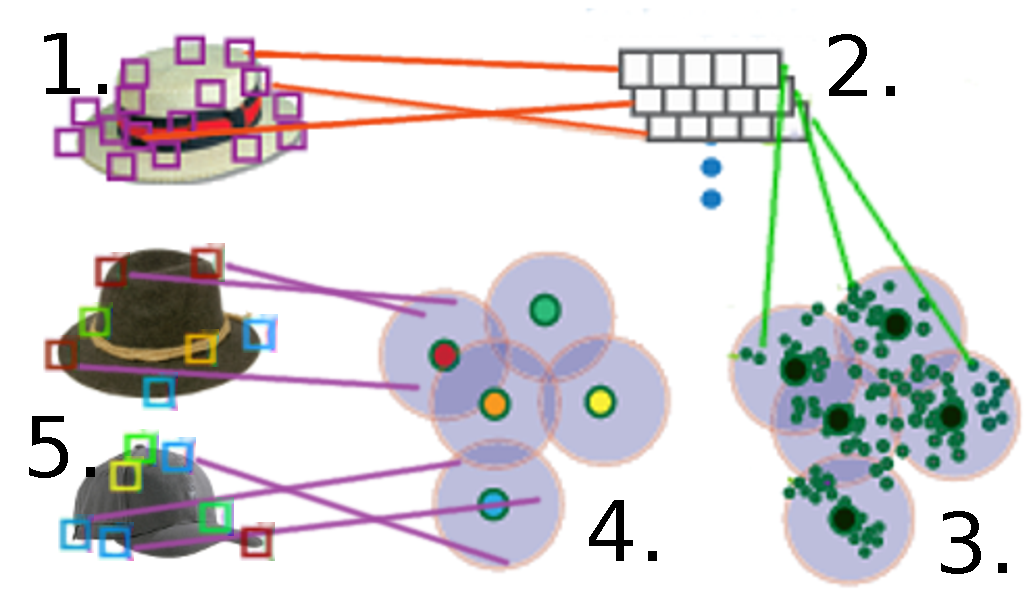
\includegraphics[width=0.45\textwidth]{baseline-system}
	\caption{Visual depiction of the baseline system. Steps: 1. Find SIFT/SURF
	keypoints. 2. Extract descriptors. 3. Cluster with K-means. 4. Create visual words
	vocabulary. 5. Calculate bag-of-words feature vectors and classify with SVM.}
\end{figure}


\section{RESULTS AND DISCUSSION}
\label{sec:results}

Results for each system can be found in \textbf{Table 2}. On the unambiguous 80x80 data
set, near-perfect results are observed by all systems. (Occasionally, an "unlucky'
training/test split would cause a single error in a trial.)  For the more complicated
non-uniform super-pixels, ScatNet is outperformed by all three baseline systems as
well has human evaluation.

We are unsure about the exact reason for ScatNet’s poorer performance in the latter
case. ScatNet is originally configured to use for uniformly sized rectangular images,
which ours aren't, so perhaps the approximate normalization method used, needs more
improvement. That ScatNet in general is suitable to the problem is evidenced by the
high performance on the uniformly sized 80x80 images. Another possibility is that,
because we only ran each configuration once in the initial filtering, our
hyper-parameter evaluation failed to identify the optimal set of parameters well.
ScatNet is very sensitive to hyper-parameter values, so it is possible that a more
optimal configuration would improve significantly. 

On the other hand, our SIFT baseline performed better than we expected, outperforming
even our human evaluation in the dataset with non-uniformly sized images. We think
both the SIFT as well as the ScatNet systems be worth comparing more directly to
the accuracy of a system with features manually designed by experts \cite{Beck2011},
which was evaluated on a different dataset. 

Finally, it is worth mentioning that every system seems to improve from using HSV
values over just the intensity values except for the SIFT baseline. Perhaps this
is due to reaching the limit of what can be classified in this data set. The
remaining images may simply be too mixed to be classified accurately by any system. 

\section{FUTURE WORK}
\label{sec:page}

If the problem leading to poor performance with ScatNet is the normalization method,
some of the following approaches could be adopted. One method could be to divide the input
image into portions of a predetermined fixed size (80 x 80, say), run ScatNet
independently on them and then generate a combined result based on the results
for each portion. Another method could be to run ScatNet on a white image of the
same size and shape (found by detecting the boundary of the input image), and
then normalize based on the sum of all the feature values.

If on the other hand the problem is our hyper-parameter choices, we could do K-fold
cross-validation instead of randomly generating the validation set for each case.
To reduce the computational burden resulting from this, we could do a
coarse-exploration of the space, followed by a hill-climbing algorithm to
find a (locally) optimal set of parameters. 

\begin{table}
	\begin{tabular}{ c | c c c }
		\multicolumn{1}{c}{Features + Algorithm} & 80x80 & Gray-SP & Color-SP \\ \hline
		SURF Descriptors + SVM & 98.2 & 86.4 & 90.2 \\ 
		SIFT Descriptors + SVM & 99.6 & \textbf{92.4} & \textbf{92.6} \\ 
		ScatNet + Affine PCA & \textbf{99.9} & 75.0 & 86.0 \\ 
		Hue v. Saturation + GMM & 98.5 & -- & 91.0 \\ 
		Human Evaluation & 100.0 & 84.0 & 89.0 \\ 
	\end{tabular}
	\caption{Accuracies of all tested systems. Best (non-buman) performers for
	each category are in bold.}
\end{table}

Our method of handling color did help most of the systems tested, though not
the accuracy of the SIFT baseline. Perhaps for this system it would be helpful
to use a variant of SIFT that inherently takes color into account, such as the algorithms
mentioned in \cite{Fan2009} or \cite{Sande2010}. It is possible that the techniques
developed in these papers could also apply to our ScatNet system. 

One more difference between the ScatNet system and the baseline is the classifier
used. It would be informative to try the PCA affine classifier on the baseline
system, and the SVM classifier on the ScatNet system to see what kind of impact
the classifier has on the result. 

Since we found that the dataset had many images that were ambiguous even to
humans, it may be helpful to either add a third category representing a mixture
and re-label the confusing images, or to add some sort of score to represent how
“mixed” the image is, and change this into a regression problem rather than a
classification problem. 

% To start a new column (but not a new page) and help balance the last-page
% column length use \vfill\pagebreak.
% -------------------------------------------------------------------------
%\vfill
%\pagebreak

% References should be produced using the bibtex program from suitable
% BiBTeX files (here: strings, refs, manuals). The IEEEbib.bst bibliography
% style file from IEEE produces unsorted bibliography list.
% -------------------------------------------------------------------------
\bibliographystyle{IEEEbib}
\bibliography{strings}

\end{document}
